%\documentclass[11pt,a4paper,runningheads]{llncs}
\documentclass[11pt,a4paper]{article}
%encoding
%--------------------------------------
\usepackage[T1]{fontenc}
\usepackage[utf8]{inputenc}
%--------------------------------------

%Portuguese-specific commands
%--------------------------------------
\usepackage[portuguese]{babel}
%--------------------------------------

%Hyphenation rules
%--------------------------------------
\usepackage{hyphenat}
\hyphenation{mate-mática recu-perar}
%--------------------------------------

\usepackage{graphicx}
\usepackage{comment}
\usepackage{pgfplots}
\usepackage{amsmath,amssymb,amsfonts}
\usepackage{algorithmic}
\usepackage{graphicx}
\usepackage{textcomp}
\usepackage{xcolor}
\usepackage{adjustbox}
\usepackage{float}
\usepackage[colorlinks=true,urlcolor=blue,linkcolor=black]{hyperref}
\usepackage[scaled]{uarial}
\renewcommand*\familydefault{\sfdefault} %% Only if the base font of the document is to be sans serif


\begin{document}

\title{Relatório Preliminar}
\author{Pedro Carrega, nº49480 \and
Vasco Ferreira, nº49470 \and Ye Yang, nº 49521
}

%\institute{Departamento de Informática da Faculdade de Ciências da Universidade de Lisboa
%\email{\{fc49480,fc49470,fc49521\}@alunos.fc.ul.pt}}

\maketitle

\renewcommand*\contentsname{Indíce}
\tableofcontents
\newpage

\section{Motivação para Dataset e Serviços}

O dataset Ecommerce foi escolhido pelo grupo devido ao grande número de eventos gerados e consequente informação produzida durante a utilização de uma loja de ecommerce. Informação esta que pode ser utilizada de diversas formas através de um grande número de variados serviços. Essa mesma informação poderá ser utilizada em vários contextos, sendo que escolhemos os seguintes 5 serviços que demonstram diferentes tipos de informação sobre o dataset:

\begin{itemize}
  \item api/products/listCategories: Fornece todas as diferentes categorias presentes nos dados
  \item api/products/popularBrands: Fornece a contagem de eventos associados a cada marca
  \item api/products/salesByBrand: Lista o numero de vendas de cada marca
  \item api/products/salePrice: Calcula o valor médio de venda de uma determinada marca
  \item api/events/ratio: Apresenta a distribuição relativa de cada tipo de evento, havendo os possíveis valores: view, cart e purchase
\end{itemize}

Os serviços foram escolhidos de forma a que consigam fazer diferentes tipos de operações sobre os dados, desde serviços mais específicos e por isso com menos carga na base de dados, a serviços mais abrangentes e consequente aumento de carga. Foram também escolhidos pois todos os serviços fornecem dados úteis para serem explorados no contexto de lojas de ecommerce.

\section{Diagrama de Casos de Uso}
\begin{figure}[H]
  \centering
    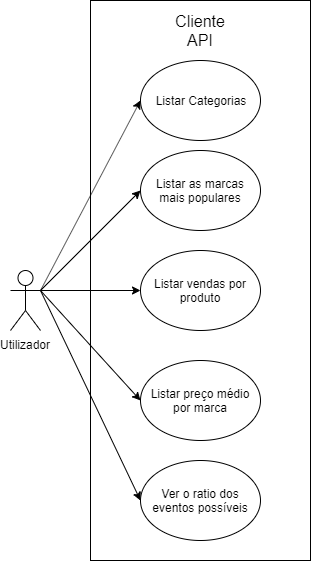
\includegraphics[scale=0.38]{Use_Cases.png}
  \caption{Diagrama de casos de uso}
\end{figure}

\section{Requisitos}

\begin{table}[H]
	\begin{center}
		\begin{tabular}{|p{3.8cm}|p{8.2cm}|}
		\hline
			\textbf{Requisitos\newline Funcionais} & \textbf{Descrição}\\ \hline
			Listar\newline Categorias Disponíveis & Serviço que fornece aos clientes todas as categorias \\ \hline
			Visualizar\newline Popularidade das\newline Marcas & Serviço que fornece cada marca associada com a sua popularidade\\ \hline
			Visualizar\newline Número de Vendas\newline Individuais & Fornece o numero total de vendas de cada marca\\ \hline
			Visualizar\newline Preço Médio de Venda & Fornece o preço médio dos produtos vendidos de uma determinada marca \\ \hline
			Visualizar\newline Rácio de Tipo\newline de Eventos & Fornece a percentagem de cada tipo de evento \\ \hline
	\end{tabular}
	\label{tab2}
	\end{center}
	\caption{Requisitos Funcionais}
\end{table}

\begin{table}[H]
	\begin{center}
		\begin{tabular}{|p{3.5cm}|p{8.5cm}|}
		\hline
			\textbf{Requisitos\newline Não Funcionais} & \textbf{Descrição}\\ \hline
			Portabilidade & Implementação de servidor em NodeJS e cliente em HTML de modo a facilitar o processo de mudança de plataforma do serviço \\ \hline
			Legibilidade & A separação clara entre as camadas de apresentação, lógica de negócio e acesso à base de dados irá tornar o fluxo do sistema mais legível para os desenvolvedores \\ \hline
			Estabilidade & A distribuição do sistema por diversas máquinas virtuais, que poderão estar distribuídas por diferentes fornecedores cloud e em diferentes Data Centers permitem obter um sistema estável \\ \hline
			Elasticidade & O sistema deverá ser capaz de se adaptar à carga de trabalho através do provisionamento e desprovisionamento dos recursos de forma autónoma. Idealmente, de forma que em qualquer ponto do tempo, o sistema apenas utilize o número de máquinas necessárias de forma a corresponder à carga atual \\ \hline
			Escalabilidade & Capacidade do sistema lidar com o crescimento de carga de trabalho. Pode-se associar à capacidade de elasticidade do sistema \\ \hline
			Confiabilidade & Visto o sistema estar implementado na núvem, conseguimos garantir alta confiabilidade nos sistema, pois se um servidor no datacenter falhar, conseguimos facilmente migrar a VM para outro servidor funcional \\ \hline
	\end{tabular}
	\label{tab1}
	\end{center}
	\caption{Requisitos Não Funcionais}
\end{table}

\section{Arquitetura da aplicação}
\begin{figure}[H]
  \centering
  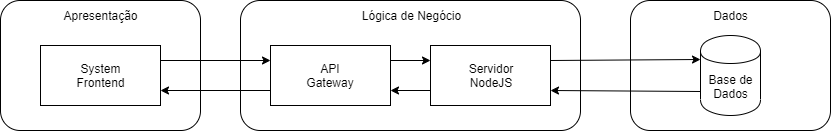
\includegraphics[scale=0.4]{App_arc.png}
  \caption{Arquitetura da aplicação}
\end{figure}

Após a definição da API na fase anterior, foi implementado de raiz um servidor em NodeJS que segue a API definida.


\subsection{Load Balancer}
Foi implementado um Load Balancer utilizando o Ingress que distribui os pedidos HTTP recebidos dos clientes browser e que reencaminha para os respetivos serviços.

\subsection{Servidores NodeJS}
Os servidores irão receber os pedidos a partir do Load Balancer, e processá-los de acordo com a funcionalidade pretendida. A lógica de negócio é aqui tratada, realizando as queries necessárias para a base de dados. Ao receber os dados, processa-os de acordo com a funcionalidade, e encaminha o resultado para o Load Balancer.
%\newline %removam isto se nao gostarem do espaço k adiciona

\subsection{Base de dados}
A base de dados está contida num containder de MongoDB dentro do qual se encontra todo o conteúdo do ficheiro .csv da base de dados anteriormente escolhida.

\subsection{Serviços Spark}
Os serviços spark também são executados no kubernetes, porém estes usam uma série de APIs e serviços diferentes fornecidos pelo GCP que irão ser apresentados mais à frente.

\section{Arquitetura técnica}
Para garantir os requisitos não funcionais mencionados a cima devemos ter em atenção os serviços da cloud escolhidos, pois proporcionam vários aspetos fundamentais dos requisitos.
\newline

A utilização dos serviços disponibilizados pelo GCP permite cumprir alguns dos requisitos não funcionais mencionados, nomeadamente a Escalabilidade e a Elasticidade. Já o Load Balancer implementado com o Ingress permite que este serviço da cloud trate automaticamente da separação dos diferentes tipos de pedidos HTTP recebidos para os respetivos serviços. A base de dados utilizada consiste numa imagem Docker baseada na imagem Mongo que como o nome sugere é uma imagem de MongoDB. Foi escolhida esta alternativa de forma a não estar dependente dos serviços de Bases de Dados de um fornecedor específico, sendo que com esta opção a imagem pode ser implementada numa instância em qualquer fornecedor cloud. Quanto à escalabilidade a imagem poderia ser replicada por diversas réplicas de forma a distribuir os pedidos feitos.
\newline

A Confiabilidade do sistema também é melhorada com a instalação em serviços na cloud, visto estas terem deteções automáticas de falhas de servidores, possibilitando a migração do sistema virtualizado para outro servidor funcional.
\newline

A Estabilidade é garantida nas várias ferramentas usadas na instalação do sistema. O Load Balancer como referido anteriormente faz a distribuição dos pedidos HTTP para os respetivos serviços, sendo que o Kubernetes atribui um DNS igual para todas as réplicas do serviço de maneira a que o Load Balancer apenas reencaminhe para o respetivo DNS, sendo o Kubernetes a distribuir a carga pelas respetivas réplicas do serviço. Isto permite que o sistema escale com facilidade já que aumentar o número de réplicas de um micro-serviço em Kubernetes é um processo rápido e sem necessitar de qualquer alteração no Load Balancer.
\newline

Já a Estabilidade é garantida devido a ter a Lógica de negócio distribuída por várias máquinas virtuais que cumprem a função de servidores.
\newline


A utilização do Docker permite-nos facilmente fazer deploy de um serviço, em qualquer máquina e em qualquer um fornecedor de cloud. Isto deve-se ao Dockerfile garantir a instalação de todas as dependências do serviço, variando conforme a linguagem de implementação do mesmo, cumprindo assim o requisito de Portabilidade do sistema.

\section{Implementação}

\subsection{Migração de AWS para GCP}
Tal como anteriormente referido o desenvolvimento dos serviços em bases portáveis tornou o processo de migração da nossa implementação prévia em AWS para GCP menos demorado, ajudando no cumprimento do deadline estipulado. As bases entre ambos os fornecedores são semelhantes, mudando apenas no caso da definição de projetos (algo que não existe no AWS) e buckets na criação de buckets de armazenamento.

\subsection{Base de dados}
A base de dados utilizadas pela aplicação básica (serviços REST) não sofreu alterações na implementação desta fase. Porém o acesso aos dados da base de dados tornou-se diferente no caso dos serviços Spark.

Dado as limitações do PySpark em conectar e ler através de um MongoDB docker container, optamos pela leitura direta do ficheiro \textbf{.csv} dentro de um bucket privado. Para tal foi necessário através do \textit{script} de inicialização a criação de um novo bucket num projeto do utilizador, dentro do qual é importado o ficheiro da base de dados, acedido através de um bucket publicamente disponível. Assim todas as leituras e escritas dos serviços Spark serão feitas de e para este novo bucket criado. Isto implica a necessidade de certas permissões para que um dado serviço num container consiga aceder ao bucket. Estas permissões são geradas no correr do \textit{script} de inicialização, que cria uma nova conta admin e exporta o ficheiro dos credenciais para ser utilizado nos vários serviços.

\subsection{Web Server}
\subsubsection{Serviços REST}
O Web Server foi inicialmente implementado em NodeJS com um router Koa. Porém a documentação relativa ao router era escassa em comparação a outras alternativas, razão pela qual mudamos para um router Express que se encontrava com melhor documentação.

As queries para a base de dados na DynamoDB foram implementadas em NodeJS, onde foi necessário tratar da paginação. A documentação relativa à paginação das queries encontrava-se disponível sendo a implementação relativamente simples, excluindo as tentativas de melhorar o desempenho.

Mudando a implementação da base de dados para uma de MongoDB, deparamo-nos com pequenos problemas de implementação das queries, mas que foram eventualmente resolvidos, observando-se um aumento de desempenho a várias ordens de magnitude em comparação com a implementação na DynamoDB (queries que demoravam 10-15 minutos na Dynamo não excediam os 20 segundos no mongo).

\subsubsection{Serviços Spark}
Para os serviços Spark, foi feita a leitura direta ao ficheiro que contém os dados do dataset como anteriormente referido. Esta implementação foi adotada pois assumimos que os serviços Spark sendo mais computacionalmente intensivo, e pela natureza dos serviços em si (estudo de dados) não irão ser executados regularmente ao contrário dos serviços REST. Assim podemos limitar as velocidades de acesso à base de dados mas mantendo o poder computacional.

Cada serviço Spark utiliza os APIs e bibliotecas NodeJS fornecidas pelo GCP, sendo necessário os credenciais corretos para qualquer mudança sobre um projeto GCP. De seguida encontra-se um diagrama da execução de um serviço spark:

\begin{figure}[H]
  \centering
  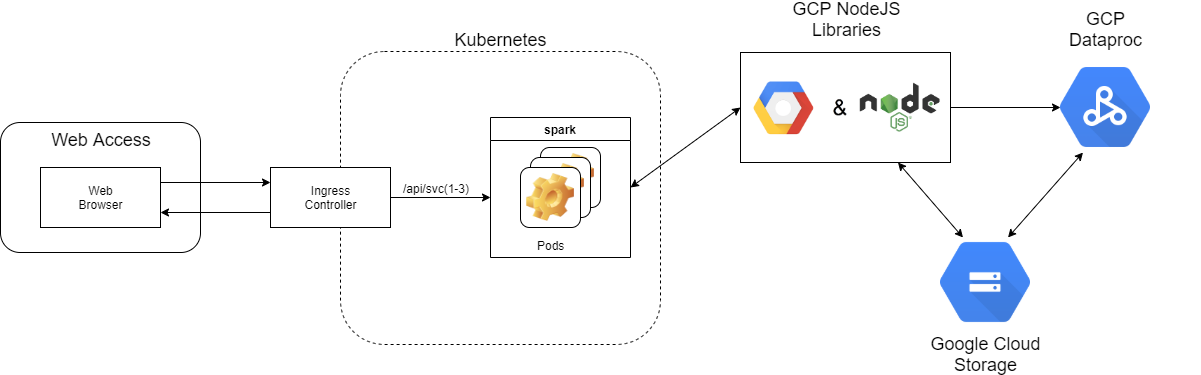
\includegraphics[scale=0.32]{spark_ex.png}
  \caption{Execução dos serviços Spark}
\end{figure}

Os serviços no backend sempre que invocados utilizam a biblioteca de NodeJS do GCP para a criação de um cluster de Dataproc, ao qual irá ser submetido o \textit{job} correspondente a cada um dos serviços. Estes \textit{jobs} acedem diretamente ao ficheiro \textbf{.csv} dentro do \textit{storage bucket} criado pelo \textit{script} a partir do qual fazem as leituras e o processamento necessário. 

Após a finalização da computação, os dados são escritos para o mesmo \textit{storage bucket} que são finalmente lidos pelo serviço NodeJS utilizando uma API de acesso ao \textit{storage} da Google Cloud.

\subsection{Limitações do GCP}
Durante a implementação do sistema, deparamo-nos com uma limitação nos recursos dos projetos do GCP, os quais que não estão em nosso controlo. Os recursos dados por defeito eram demasiado limitantes e os serviços de suporte da Google não permitiam o aumento dos limites devido a falta de dados de utilização visto as contas utilizadas serem recentes.

Para possibilitar o lançamento e o teste dos serviços tivemos que conglomerar os 3 serviços sparks num só o que limita a escalabilidade do sistema. Esta decisão teve de ser tomada pois não havia outra alternativa (mesmo com instâncias de tamanho mínimo dentro de um cluster) que permitisse o lançamento dos serviços REST juntamente com os serviços Spark (visto que cada serviço Spark cria um cluster \textbf{Dataproc} chegando rapidamente aos limites de IPs \textit{in-use} e número de instâncias).

\section{Consolidação do projeto}
\subsection{Terraform}
Para a entrega da fase de consolidação, decidimos tornar o processo de execução e \textit{tear-down} mais automatizada. Para tal incorporamos no \textit{script} de deployment a utilização do Terraform.

O Terraform possibilitou-nos a criação e destruição automática dos recursos criados no projeto GCP de forma a que o processo seja mais automatizado e facilitado. Comandos como \textbf{terraform init} e \textbf{terraform destroy} permitem a criação e destruição de recursos por nós definidos dando as credenciais de GCP certas. Tal é possível devido ao suporte de serviços Google por parte do Terraform que permite aceder a vários recursos da GCP e a criação dos mesmo.

\section{Execução do \textit{script}}
\subsection{Requerimentos}
Para a execução do \textit{script} assume-se que a máquina local tem as seguintes ferramentas instaladas:
\begin{itemize}
	\item Docker
	\item gcloud CLI
	\item NodeJS
	\item (Opcional para testar localmente) PySpark
	\item Terraform
\end{itemize}

\subsection{Pré-preparação}
Antes da execução do \textit{script} de deployment é necessário a criação de um projeto na conta pessoal do GCP e ativar o billing.

Dado que os dados de pagamento são confidenciais, não é possível automatizar a criação de um projeto com a validação do billing.

Após criado o projeto, guardar o \textbf{project-id} atribuído.

Após criado o projeto no GCP, navegar para o ficheiro \textbf{deploy-gcp.sh} e abrir o ficheiro. Editar apenas as seguintes variáveis de ambiente definidas no ficheiros: \textbf{PROJECT\_NAME} (com o id anteriormente atribuido), \textbf{BUCKET \_NAME} (um nome para um \textit{storage bucket} único) e \textbf{CLUSTER\_NAME}.

\subsection{Deployment do sistema}
Para executar o script basta inserir no terminal: \textbf{./deploy-gcp} e seguir os passos de autenticação que irão ser pedidos.

O script irá tratar da escrita dos ficheiros de inicialização de recursos usando o Terraform, a criação e exportação dos credenciais necessários para acesso aos serviços da GCP, a escrita, montagem e deployment em containers do código fonte da camada de negócio e finalmente a criação dos pods que irão conter todos os serviços e o load balancer no cluster de Kubernetes criado.

\subsection{Acesso ao serviço}
Após a finalização do script de deployment, haverá um tempo de espera de cerca de \textbf{5 minutos} até que o load balancer criado acabe de realizar todos os health checks necessários. O estado dos health checks pode ser verificado com o seguinte comando:
\begin{itemize}
	\item \textbf{kubectl describe ingress}
\end{itemize}

Após a terminção dos health checks (mensagem OK) é possível aceder aos serviços utilizando o IP gerado. O IP pode ser retirado utilizando o comando anterior, ou alternativamente através do seguinte comando:
\begin{itemize}
	\item \textbf{kubectl get ingress}
\end{itemize}

Para aceder um serviço basta colocar o endereço IP num navegador web ou no Postman com pedido GET e completando com os URLs definidos no nosso API (ex.: <ip-add>/api/spark/svc1).

\subsection{Desconstrução do deployment}
Para apagar os recursos criados basta seguir os seguintes passos:
\begin{itemize}
	\item Navegar para a diretoria do terraform criada pelo script e correr no terminal: \textbf{terraform destroy}, esperar pelo fim da execução
	\item Navegar para a \href{http://console.cloud.google.com/}{consola} do gcp e apagar o projeto inicialmente criado
	\item Eliminar as imagens docker locais executando \textbf{docker images} para obter os IDs de todas as imagens e \textbf{docker image rm <ID1 ID2 ... IDN>} para remover todas as imagens. 
\end{itemize}

\section{Cenários de Validação}	
\begin{itemize}
	\item Listar Categorias:
	\begin{enumerate}
		\item Inserir no navegador o URL anteriormente mencionado acrescentado \textbf{/api/products/listCategories}
		\item Após alguns segundos irá aparecer no ecrã o resultado.
	\end{enumerate}
	\item Listar a popularidade das marcas:
	\begin{enumerate}
		\item Inserir no navegador o URL anteriormente mencionado acrescentado \textbf{/api/products/popularBrands}
		\item Após alguns segundos irá aparecer no ecrã o resultado.
	\end{enumerate}
	\item Listar vendas de cada marca:
	\begin{enumerate}
		\item Inserir no navegador o URL anteriormente mencionado acrescentado \textbf{/api/products/salePrice}
		\item Após alguns segundos irá aparecer no ecrã o resultado.
	\end{enumerate}
	\item Listar o preço médio de uma marca:
	\begin{enumerate}
		\item Inserir o url mencionado posteriormente adicionado "/<Marca>", aonde <Marca> representa a marca que o utilizador quer analisar.
		\item Após alguns segundos irá aparecer no ecrã o resultado.
	\end{enumerate}
	\item Ver o ratio dos eventos possíveis:
	\begin{enumerate}
		\item Inserir no navegador o URL anteriormente mencionado acrescentado \textbf{/api/events/ratio}
		\item Após alguns segundos irá aparecer no ecrã o resultado.
	\end{enumerate}
	\item Portabilidade:
	\begin{enumerate}
		\item Escolher 2 diferentes fornecedores de serviço cloud
		\item Implementar os serviços criados, nas plataformas diferentes utilizando os docker containers fornecidos.
		\item Verficar que ambos os serviços se encontram funcionais
	\end{enumerate}

Os docker containers tornam os sistema muito portável dado que é uma ferramenta comum entre os vários fornecedores de serviços cloud. Daí o deployment dos serviços é facilitada caso seja necessário a mudança de fornecedor, sendo apenas necessário tratar dos aspetos técnicos em termos de balanceamento de carga e quantidade de instâncias ativas nos serviços utilizando as ferramentas de cada fornecedor.

	\item Elasticidade:
	\begin{enumerate}
		\item Verfique o numero de instâncias virtuais ativas
		\item Assumindo uma baixa carga de sistema, sobrecarregue o serviço com pedidos
		\item Visualize o numero de maquinas virtuais ativas aumentar de forma a poder satisfazer os diferentes pedidos sem afetar a qualidade do serviço
	\end{enumerate}
\end{itemize}

\section{Discussão e Conclusões}
Durante o desenvolvimento do projeto foram encontrados bastantes obstáculos, seja na implementação dos serviços, na escolhe e consequente aplicação da base de dados ou na automatização dos \textit{scripts} de implementação dos serviços desenvolvidos. Todos estes problemas resultaram em muitas horas de trabalho extra por parte do grupo, mas serviram também de aprendizagem, seja em como trabalhar com fornecedores de serviços na nuvem, ou como desenvolver \textit{scripts} de automatização de implementação. Apesar de todos os problemas, o grupo foi capaz de os solucionar de forma eficiente como mencionados na secção da Arquitetura técnica.

O DynamoDB aparenta ser uma boa solução para fazer hosting de bases de dados onde a procura seja limitada a um conjunto de valores limitados. Isto torna-o pouco útil para a nossa implementação, porém, continua a ser uma boa ferramenta para os casos mencionados se a base de dados for de dimensões elevadas, sendo difícil fazer o hosting local da mesma.

Os serviços da cloud no geral, se utilizadas de forma correta, aparentam ser poderosas em sentido computacional, tendo uma grande variedade de ferramentas que possibilita a implementação de aplicações, serviços ou outra qualquer funcionalidade.

Na nossa experiência pessoal, a documentação da AWS foi mais escassa em comparação ao GCP. Dado a escolha entre ambas recomendaríamos fortemente a utilização do GCP para futuras implementações.
\end{document}